% This is a LaTex template for scribe notes for 
% CS 6170: Computational Topology. 
% This template is adapted from a template thanks to 
% Jeff A. Bilmes @ U. Washington and Alistair Sinclair @ Berkeley. 

\documentclass{article}
\usepackage{times,amsmath,amsthm,amsfonts,eucal,graphicx}
\usepackage{amssymb}
\usepackage{enumitem}
\usepackage{color}
\usepackage{graphicx}
\usepackage{subcaption}
\usepackage{hyperref}
\usepackage{cleveref}

\setlength{\oddsidemargin}{0.25 in}
\setlength{\evensidemargin}{-0.25 in}
\setlength{\topmargin}{-0.6 in}
\setlength{\textwidth}{6.5 in}
\setlength{\textheight}{8.5 in}
\setlength{\headsep}{0.75 in}
\setlength{\parindent}{0 in}
\setlength{\parskip}{0.1 in}

%
% The following commands set up the lecnum (lecture number)
% counter and make various numbering schemes work relative
% to the lecture number.
%
\newcounter{lecnum}
\renewcommand{\thepage}{\thelecnum-\arabic{page}}
\renewcommand{\thesection}{\thelecnum.\arabic{section}}
\renewcommand{\theequation}{\thelecnum.\arabic{equation}}
\renewcommand{\thefigure}{\thelecnum.\arabic{figure}}
\renewcommand{\thetable}{\thelecnum.\arabic{table}}

%
% A few symbols that we will be using often in this course.
\newcommand{\indep}{{\bot\negthickspace\negthickspace\bot}}
\newcommand{\notindep}{{\not\negthickspace\negthinspace{\bot\negthickspace\negthickspace\bot}}}
\newcommand{\definedtobe}{\stackrel{\Delta}{=}}
\renewcommand{\choose}[2]{{{#1}\atopwithdelims(){#2}}}
\newcommand{\argmax}[1]{{\hbox{$\underset{#1}{\mbox{argmax}}\;$}}}
\newcommand{\argmin}[1]{{\hbox{$\underset{#1}{\mbox{argmin}}\;$}}}

%
% The following macro is used to generate the header.
%
\newcommand{\lecture}[4]{
   \pagestyle{myheadings}
   \thispagestyle{plain}
   \newpage
   \setcounter{lecnum}{#1}
   \setcounter{page}{1}
   \noindent
   \begin{center}
   \framebox{
      \vbox{\vspace{2mm}
    \hbox to 6.58in { {\bf CS 6170 Computational Topology: Topological Data Analysis
                        \hfill University of Utah} }
    \hbox to 6.58in { {\bf Spring 2017
                        \hfill School of Computing} }
       \vspace{4mm}
       \hbox to 6.28in { {\Large \hfill Lecture #1: #2  \hfill} }
       \vspace{2mm}
       \hbox to 6.28in { {\it Lecturer: {\it Prof. Bei Wang {\tt <beiwang@sci.utah.edu>}} \hfill Scribe: #3} }
      \vspace{2mm}}
   }
   \end{center}
   \markboth{Lecture #1: #2}{Lecture #1: #2}
   \vspace*{4mm}
}

%
% Convention for citations is authors' initials followed by the year.
% For example, to cite a paper by Leighton and Maggs you would type
% \cite{LM89}, and to cite a paper by Strassen you would type \cite{S69}.
% (To avoid bibliography problems, for now we redefine the \cite command.)
% Also commands that create a suitable format for the reference list.
\renewcommand{\cite}[1]{[#1]}
\def\beginrefs{\begin{list}%
        {[\arabic{equation}]}{\usecounter{equation}
         \setlength{\leftmargin}{2.0truecm}\setlength{\labelsep}{0.4truecm}%
         \setlength{\labelwidth}{1.6truecm}}}
\def\endrefs{\end{list}}
\def\bibentry#1{\item[\hbox{[#1]}]}

%Use this command for a figure; it puts a figure in wherever you want it.
%usage: \fig{NUMBER}{CAPTION}{.eps FILE TO INCLUDE}{WIDTH-IN-INCHES}
\newcommand{\fig}[4]{
			\begin{center}
	                \includegraphics[width=#4,clip=true]{#3} \\
			Figure \thelecnum.#1:~#2
			\end{center}
	}
% Use these for theorems, lemmas, proofs, etc.
\newtheorem{theorem}{Theorem}[lecnum]
\newtheorem{lemma}[theorem]{Lemma}
\newtheorem{proposition}[theorem]{Proposition}
\newtheorem{claim}[theorem]{Claim}
\newtheorem{corollary}[theorem]{Corollary}
\newtheorem{definition}[theorem]{Definition}
% \newenvironment{proof}{{\bf Proof:}}{\hfill\rule{2mm}{2mm}}

\newcommand\will[1]{\textcolor{Red}{(Will: #1)}}

% **** IF YOU WANT TO DEFINE ADDITIONAL MACROS FOR YOURSELF, PUT THEM HERE:

\begin{document}
%FILL IN THE RIGHT INFO.
%\lecture{**LECTURE-NUMBER**}{**DATE**}{**LECTURER**}{**SCRIBE**}
\lecture{23}{April 4, 2017}{Chris Brooks, Will Usher}

% **** YOUR NOTES GO HERE:

Thursday 4/6 Quiz
Given a 1 or 2 dimensional function, give reeb graph, contour tree or mapper

Topics:
Extended persistence
Elevation function
Protein Docking

\section{Extended Persistence}

There is something not satisfactory about ordinary persistence. Consider a ``deformed torus''
\cref{fig:deformed-torus} with a height function $f$. Going from bottom to top, the
sublevel sets $\mathbb{X}=f^{-1}(-\infty,a]$ are a bowl at the first local min $a$,
two bowls at the next local min $b$, glued bowls at the saddle point $c$,
a bowl with a handle at the second saddle point $d$ (note the tunnel) and so on.
As we move up the object, a tunnel is formed at $e$ which is not filled by the addition
of any subsequent critical points. This tunnel indicates an important feature about
the object, in its structure.

\begin{figure}[htb!]
	\centering
	\begin{subfigure}{0.45\columnwidth}
		\centering
		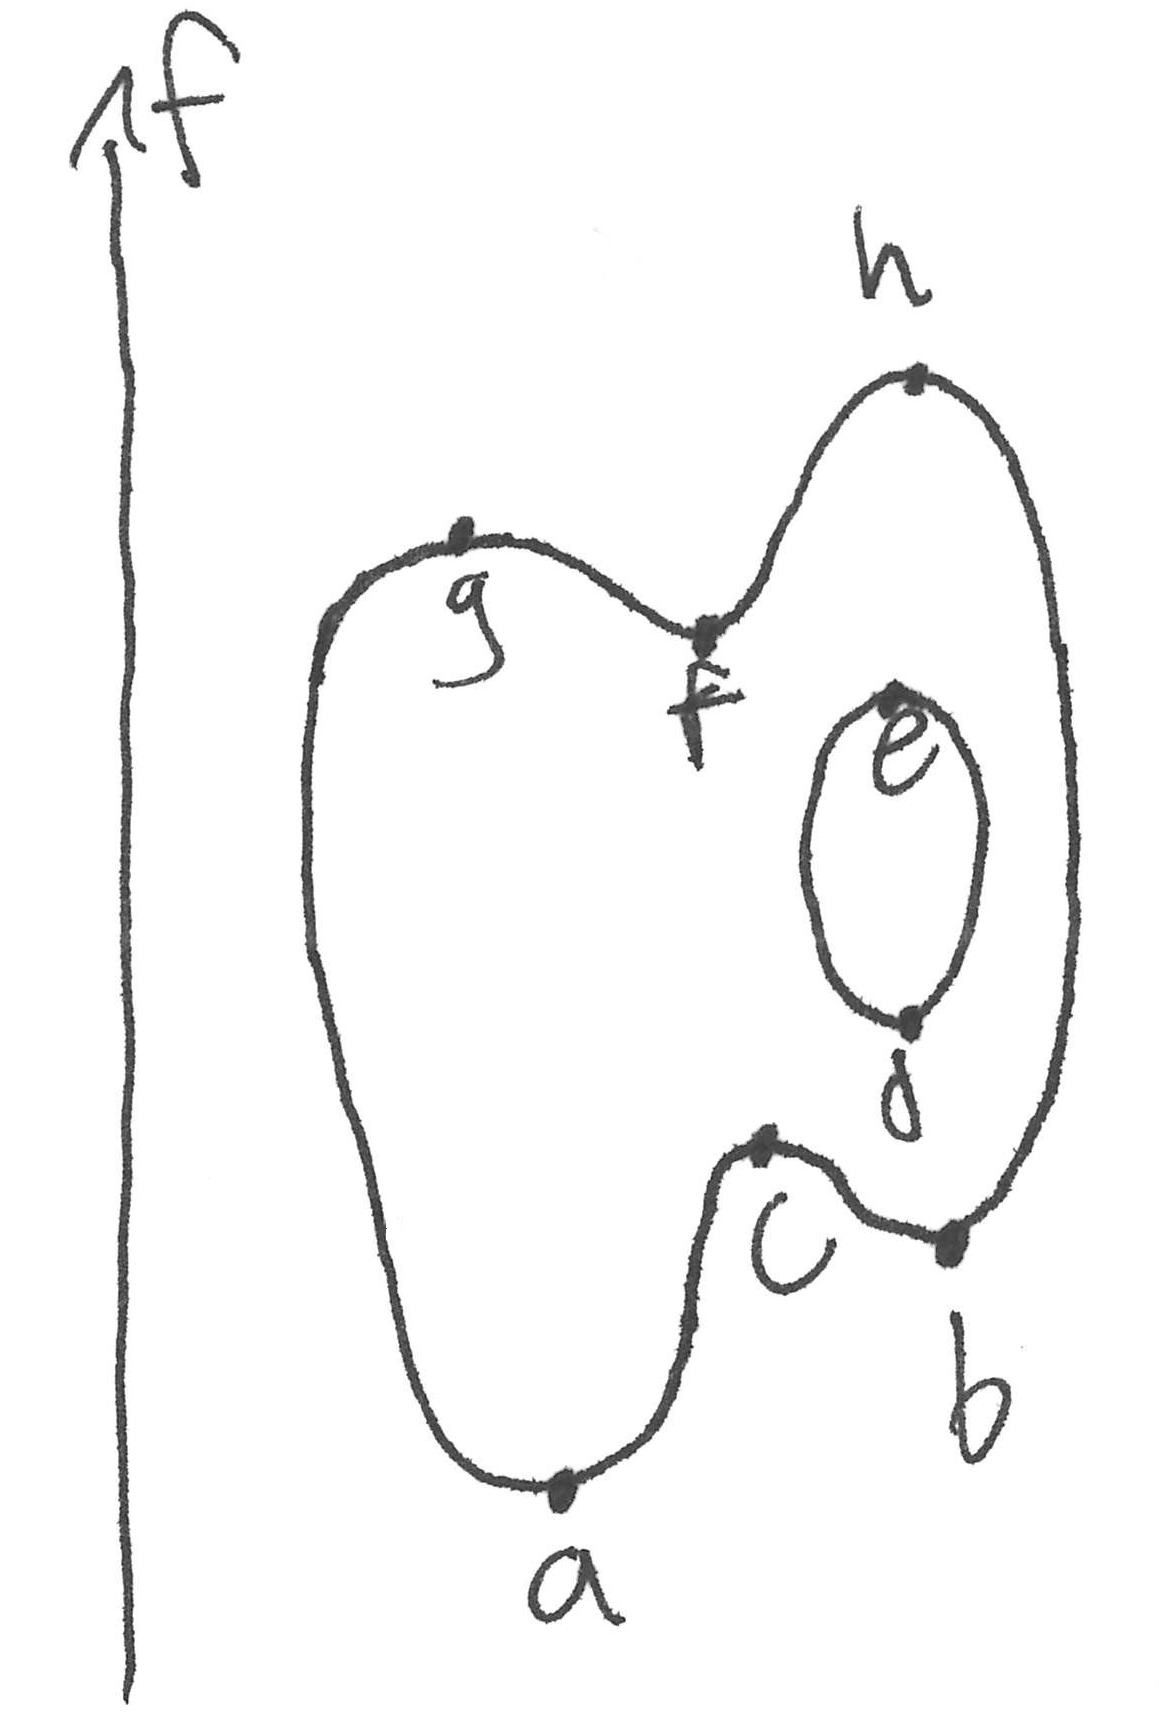
\includegraphics[height=8cm]{fig/blobby-torus}
		\caption{\label{fig:deformed-torus}}
	\end{subfigure}
	\begin{subfigure}{0.45\columnwidth}
		\centering
		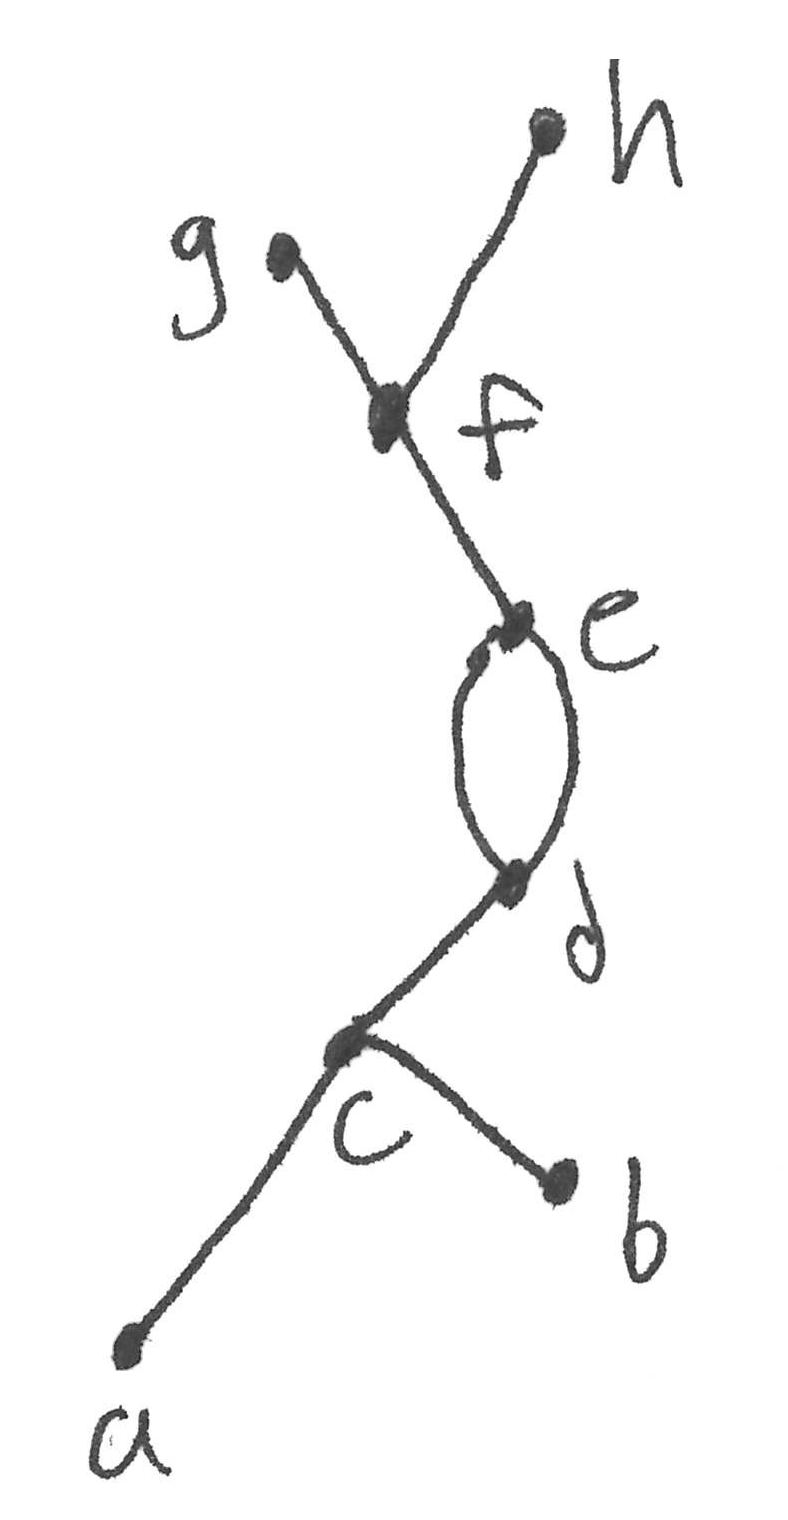
\includegraphics[height=8cm]{fig/blobby-torus-reeb-graph}
		\caption{\label{fig:reeb-graph}}
	\end{subfigure}
	\caption{\label{fig:torus-reeb} The deformed torus (a) and its Reeb graph for the
	height function $f$}
\end{figure}

We can pair critical points based on features being born at one, and killed at the next.
For example, we can pair $(b,c)$ on the basis of a component being born at $b$ and killed at $c$. Same for $(f,g)$. We can also pair the global minimum with the global maximum $(a,h)$. This is the first part of ``extended persistence'' and it captures an \emph{essential feature} of the space. We call $(a,h)$ an \emph{extended persistence pair}. Another essential feature would be the tunnel described by the pair of saddle points $(d,e)$.
These pairs are features created but not destroyed during the sub-level set filtration, and
correspond to essential features in the structure.
In the Reeb graph for this space (\cref{fig:reeb-graph}), the smallest branches correspond to the ordinary pairs, and the remaining vertices can be associated with the extended persistence pairs.
We can also do ``persistence simplification''. For example, if we push the point $b$ up to, or past $c$, we remove the two critical points, and the protrusion associated with it. This can also be done by bringing $c$ down
to $b$ or moving them both up and down to some equal height \cref{fig:simplification}.

These features of a topological space can be useful in analyzing the interaction of proteins and other molecules since these interactions are dependent on the compatibility of their shapes. The persistence pairs from the previous example give a sense of the size of that feature; for instance, the pair $(c,d)$ gives the size of the corresponding protrusion by computing the difference in height between the points $|f(d) - f(c)|$.
By comparing the persistence of the differente features on each protein we wish to dock, we can determine
the best docking orientation, or if they are incompatible.

\begin{figure}
	\centering
	\begin{subfigure}{0.24\columnwidth}
		\centering
		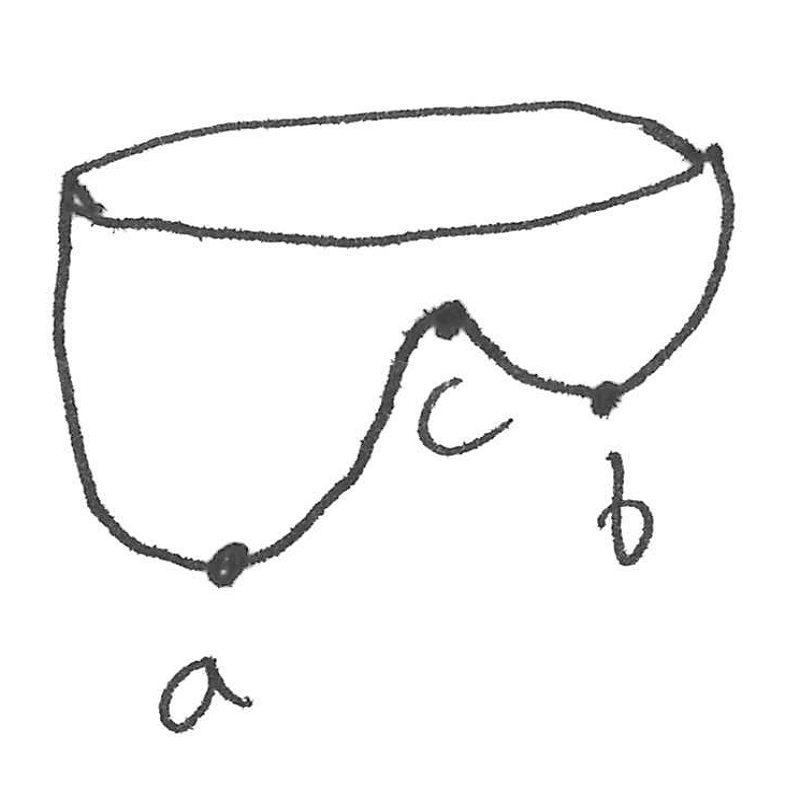
\includegraphics[width=\textwidth]{fig/blobby-torus-bottom}
		\caption{Bottom of deformed torus}
	\end{subfigure}
	\begin{subfigure}{0.24\columnwidth}
		\centering
		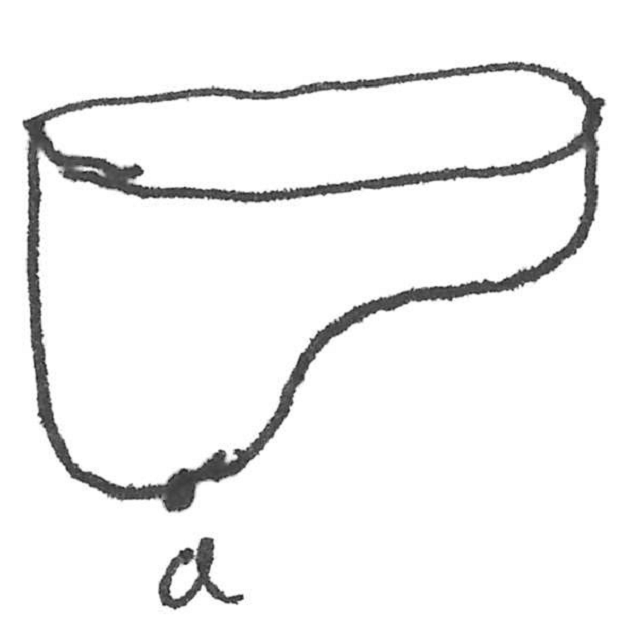
\includegraphics[width=\textwidth]{fig/blobby-torus-bottom-reduced1}
		\caption{Simplify by pushing $b$ up}
	\end{subfigure}
	\begin{subfigure}{0.24\columnwidth}
		\centering
		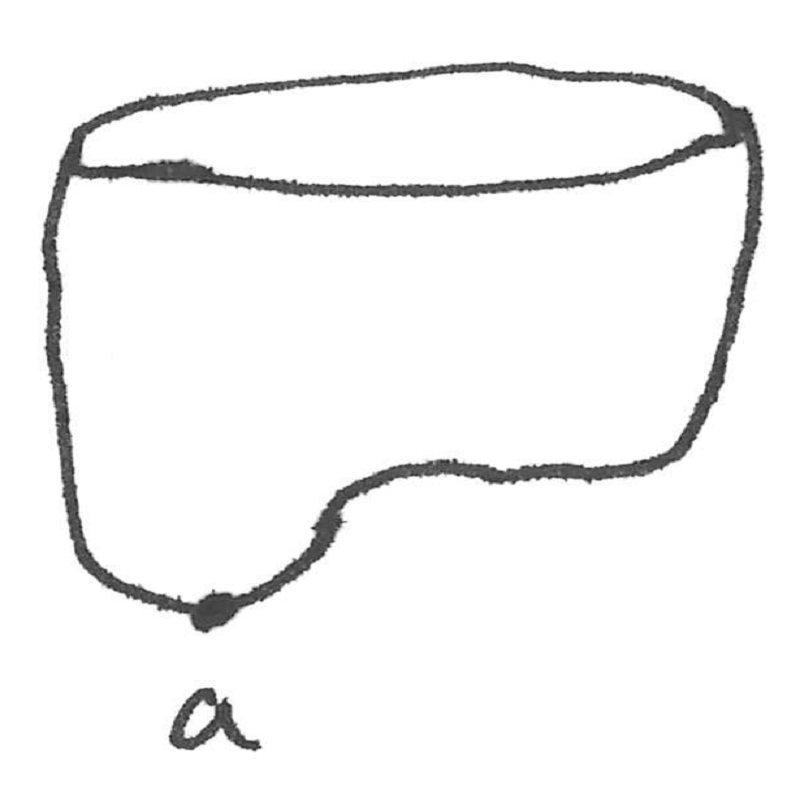
\includegraphics[width=\textwidth]{fig/blobby-torus-bottom-reduced2}
		\caption{Simplify by pushing $c$ down}
	\end{subfigure}
	\begin{subfigure}{0.24\columnwidth}
		\centering
		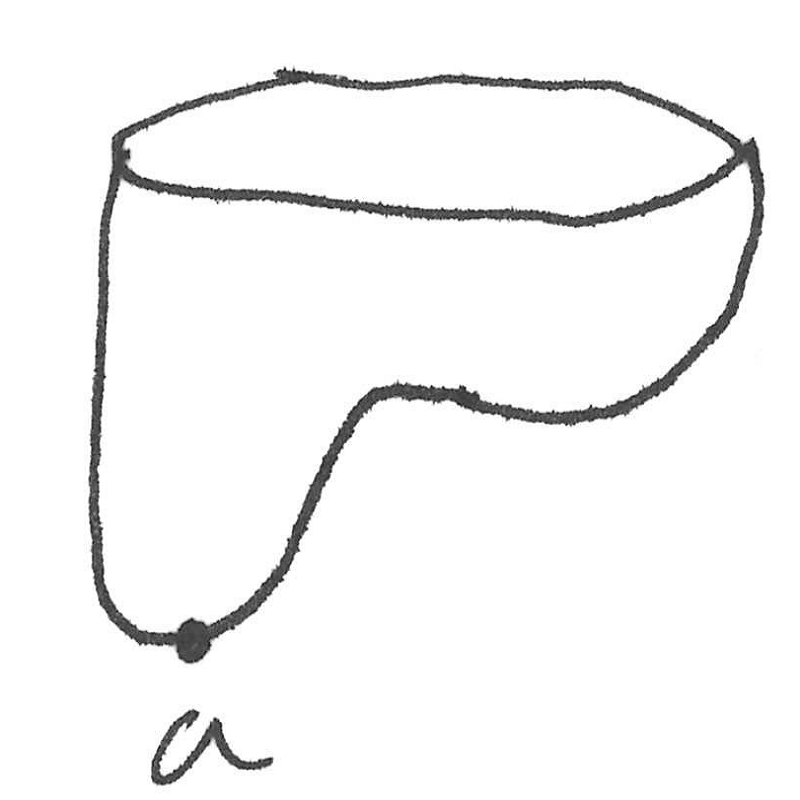
\includegraphics[width=\textwidth]{fig/blobby-torus-bottom-reduced3}
		\caption{Simplify by moving both}
	\end{subfigure}
	\caption{\label{fig:simplification} Different methods for moving the critical points $b$ and $c$
	to remove the lower-persistence feature.}
\end{figure}

\section{Elevation Function}

An elevation function $E:\mathbb{X}\to\mathbb{R}$ for any point $x\in\mathbb{X}$ gives us $E(x)$, which is the persistence of $x$ when it becomes critical. In the previous examples the critical points appeared where the normal direction aligned with the height direction. As we change the height direction, the corresponding
critical points will also change (\cref{fig:elevations}).

In the first example (\cref{fig:torus-reeb}), the elevation function $f$ is defined by $E(f)=E(g)=|t_g-t_f|$, $E(a)=E(h)=|t_h-t_a|$, etc. If our height function is not Morse, there may be multiple critical points that can be paired with another critical point. This can happen if we sample directions on a shape to do this kind of analysis; a small perturbation can eliminate the ambiguity.
As proteins can rotate and dock in different orientations we can use multiple elevation functions
in different directions to determine if they are compatible in some orientation
This gives us different critical points and new critical pairs which highlight the shape's features along that direcion.

\begin{figure}
	\centering
	\begin{subfigure}{0.32\columnwidth}
		\centering
		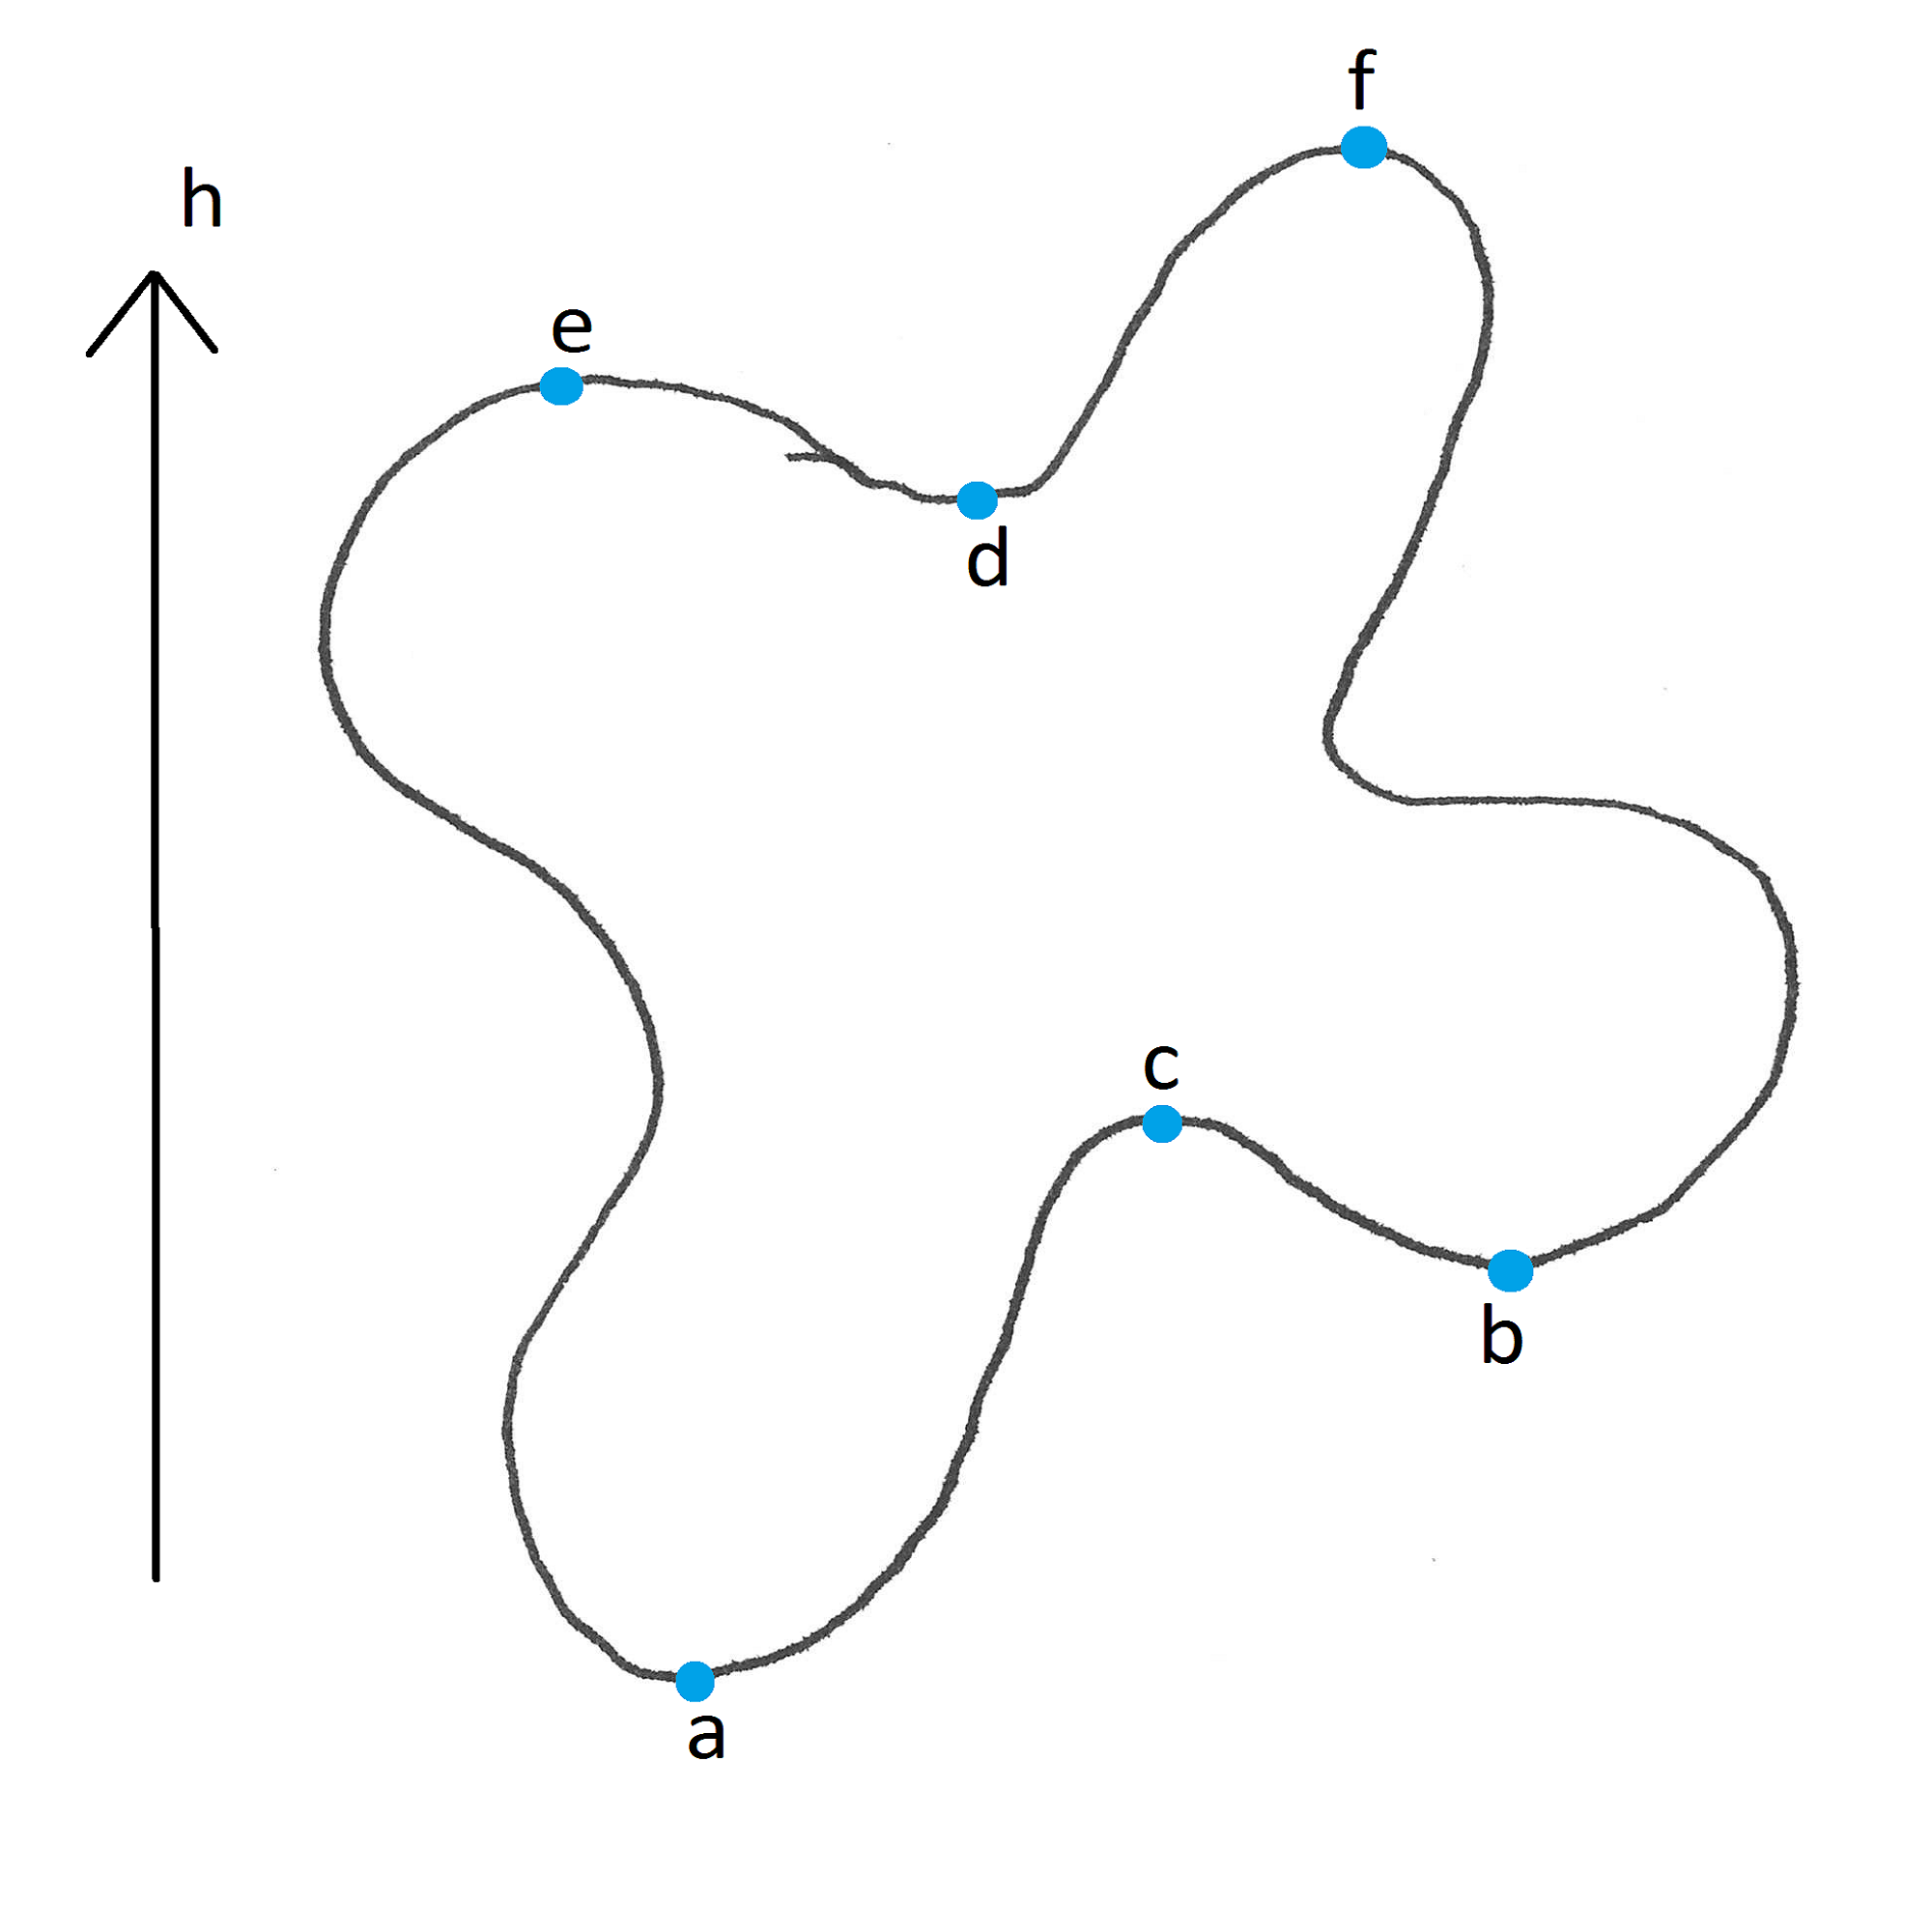
\includegraphics[width=\textwidth]{fig/blobby-molecule-h-vertical}
	\end{subfigure}
	\begin{subfigure}{0.32\columnwidth}
		\centering
		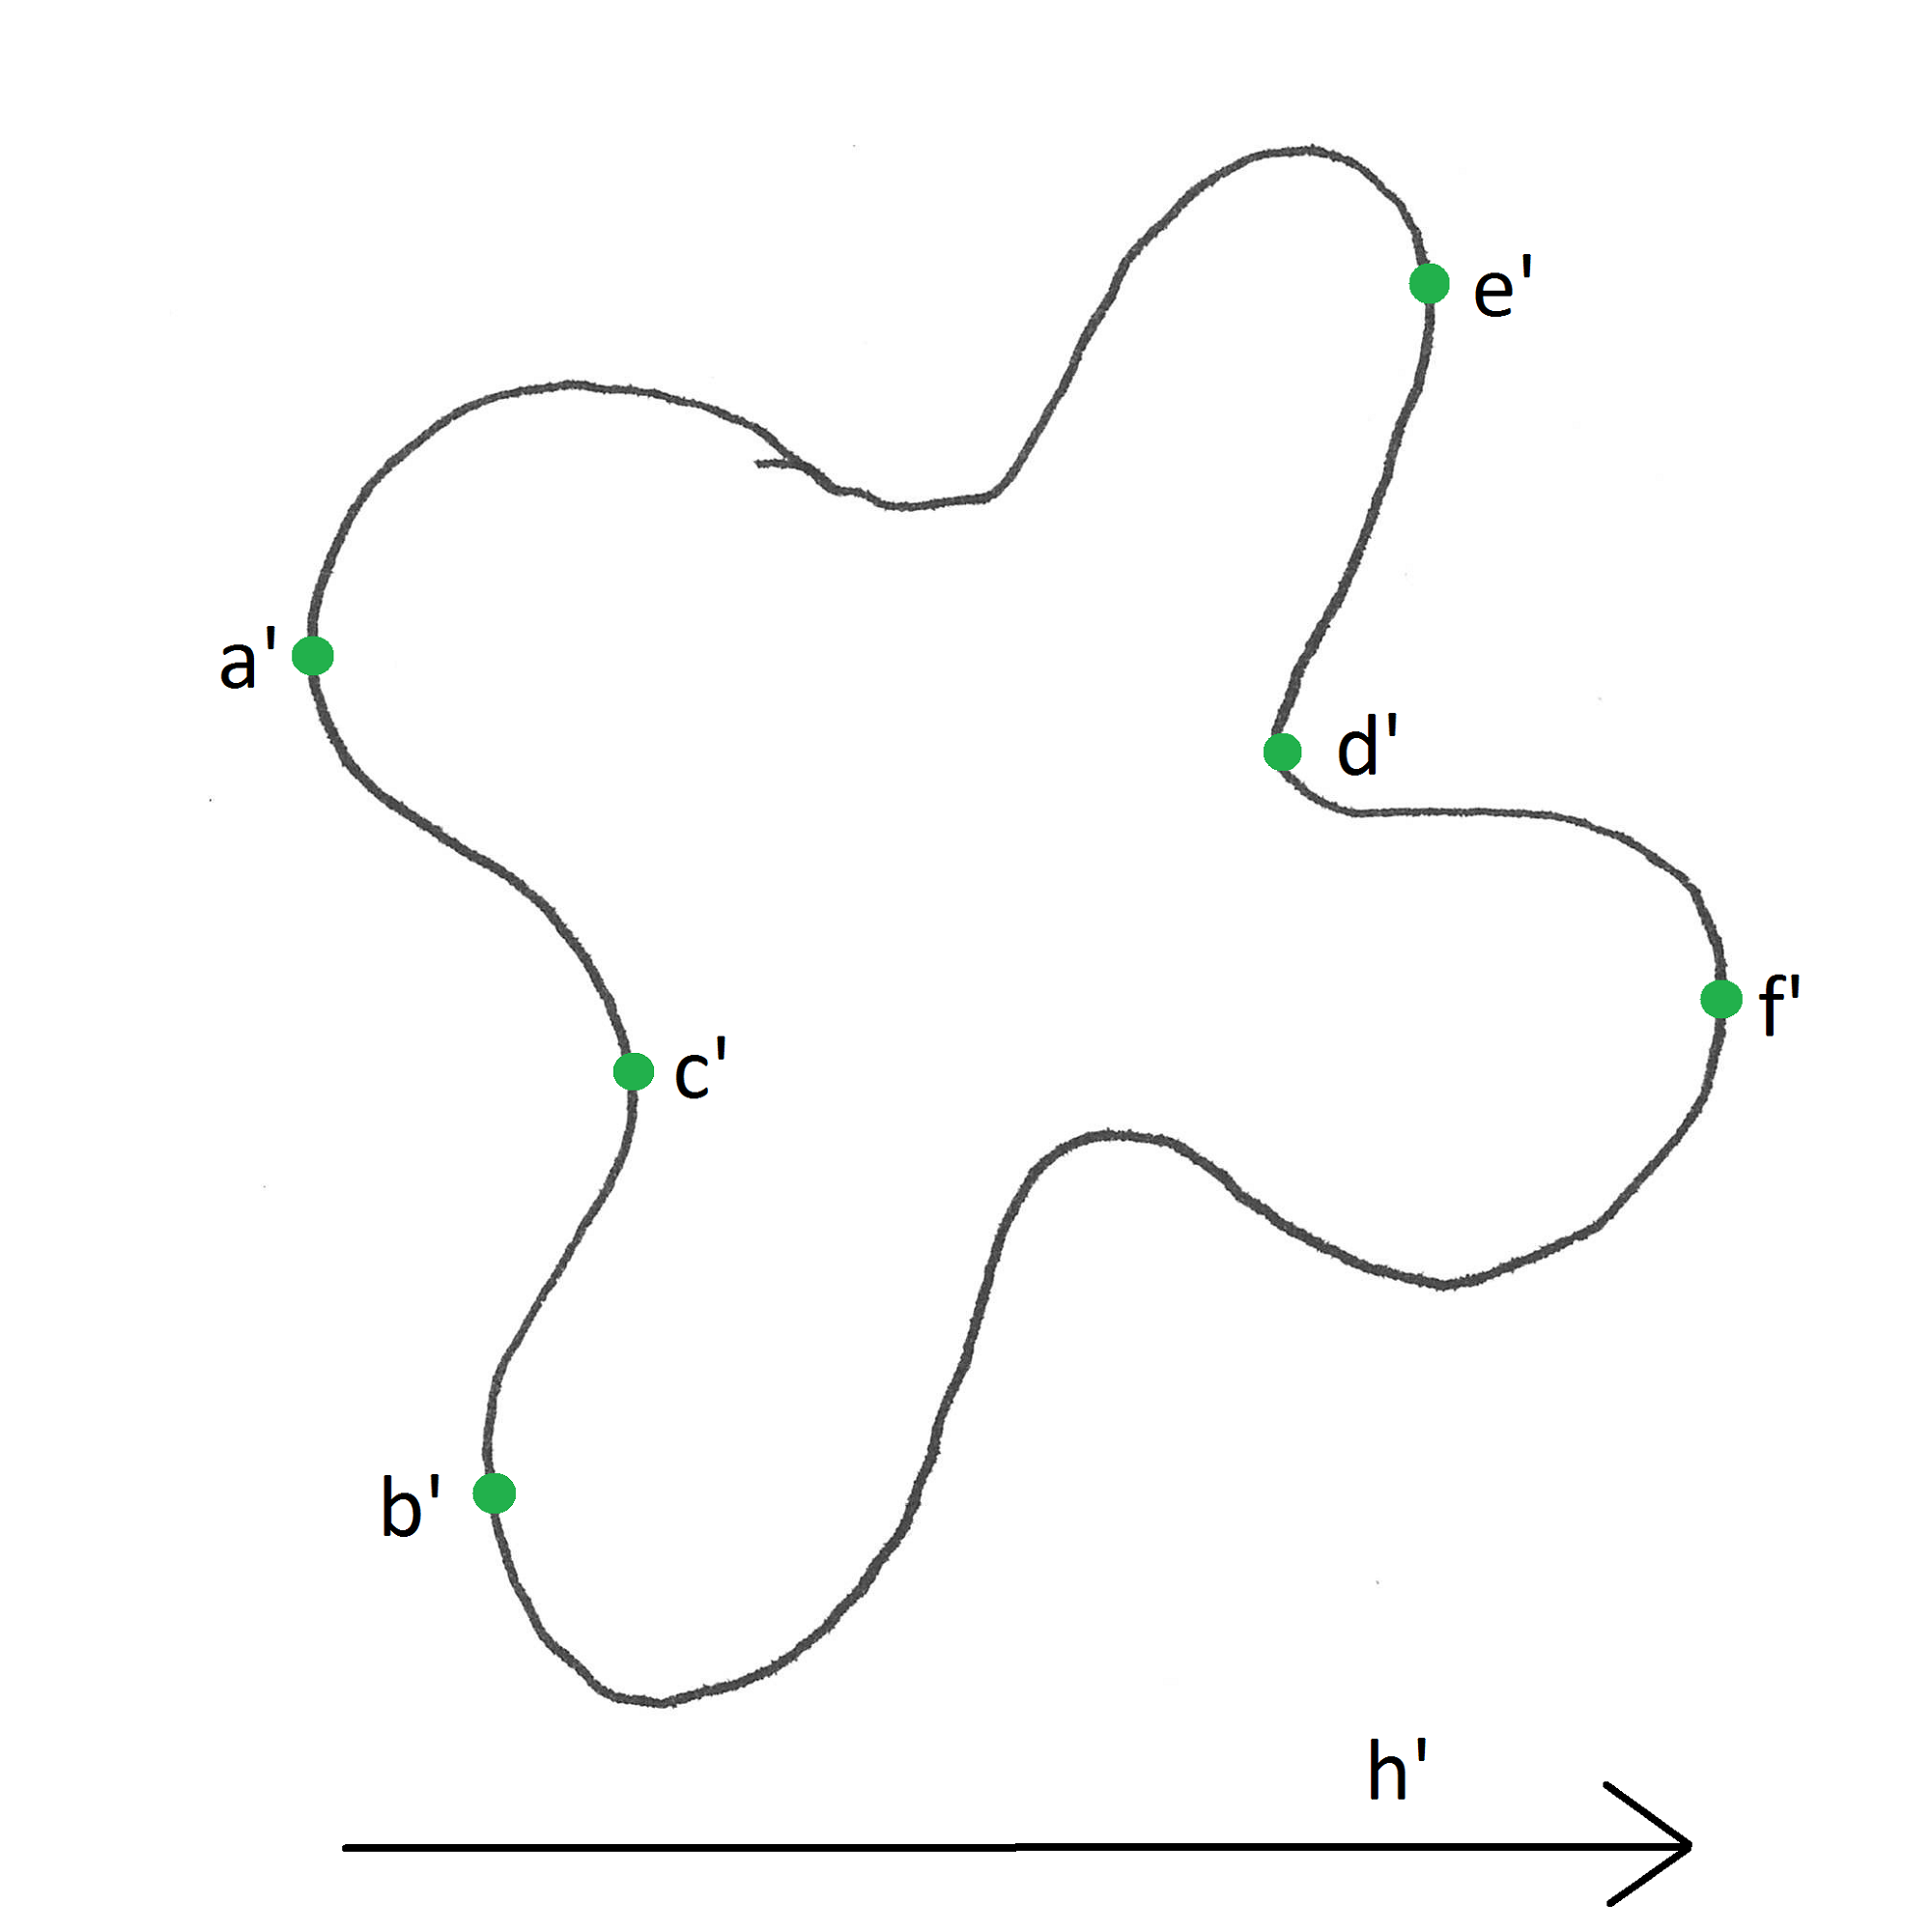
\includegraphics[width=\textwidth]{fig/blobby-molecule-h-horizontal}
	\end{subfigure}
	\begin{subfigure}{0.32\columnwidth}
		\centering
		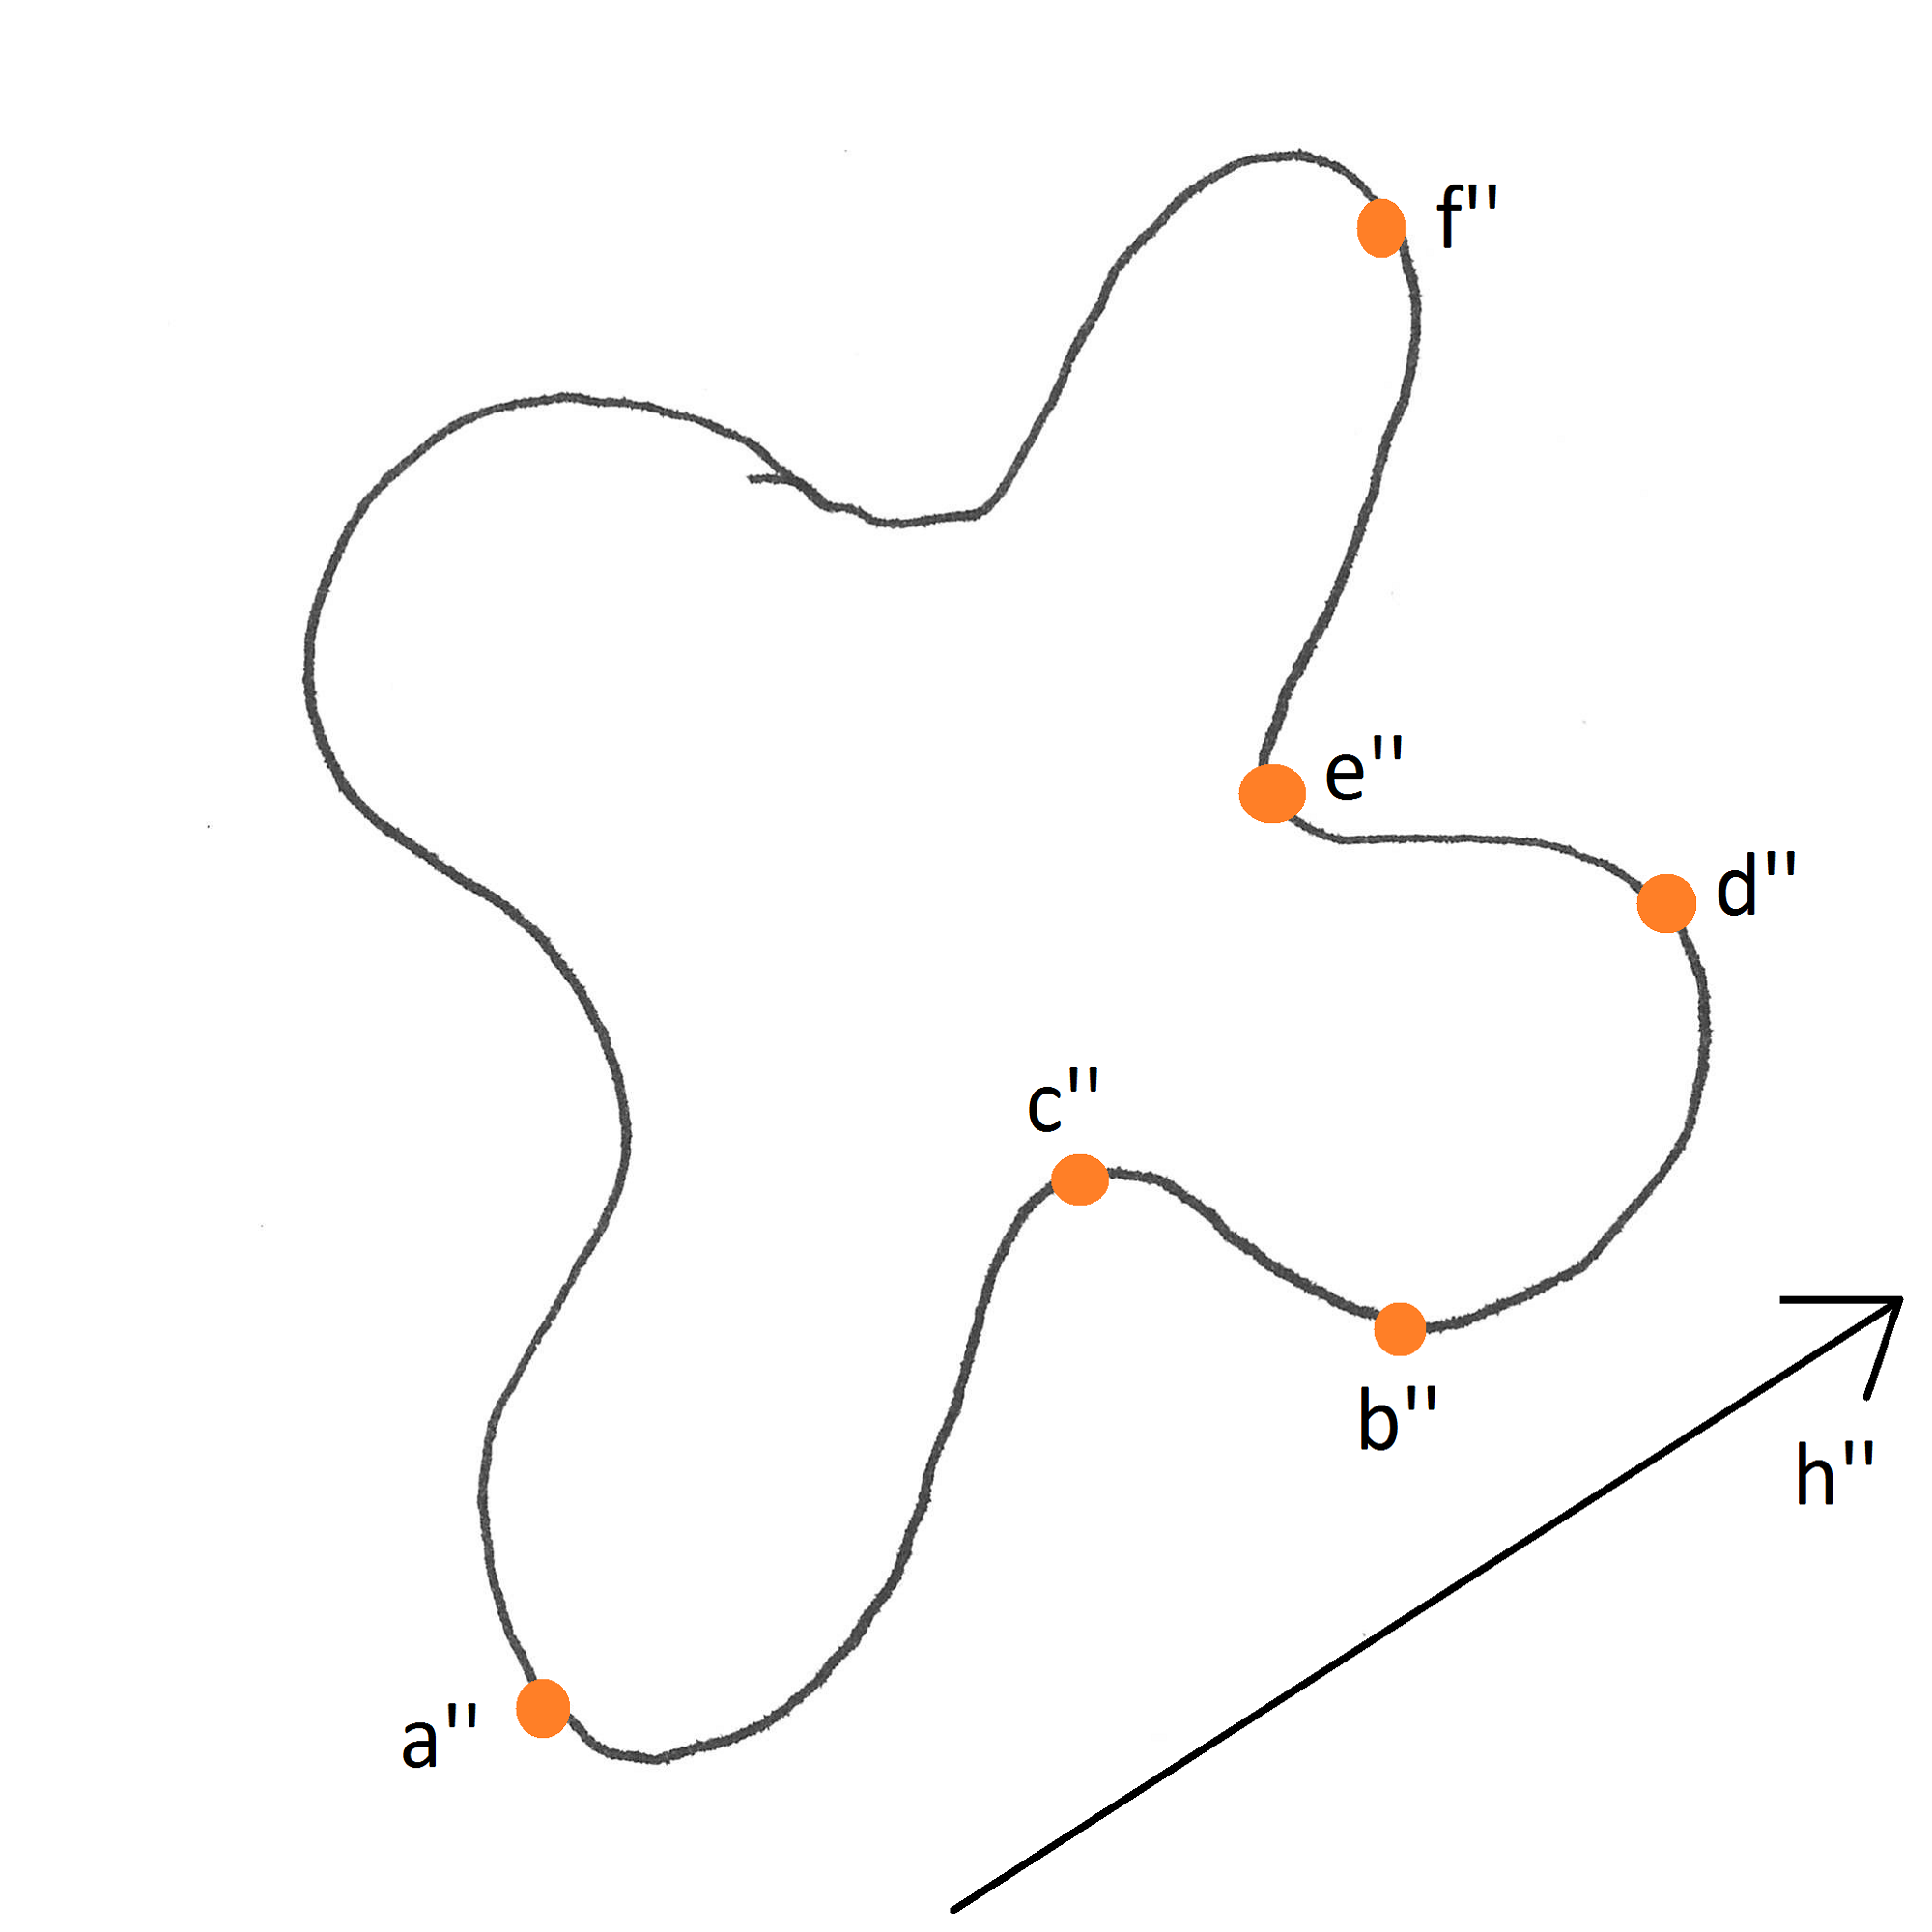
\includegraphics[width=\textwidth]{fig/blobby-molecule-h-diagonal}
	\end{subfigure}
	\caption{\label{fig:elevations} As the height function direction changes, the
	critical points change accordingly.}
\end{figure}

\section{Application to Protein Docking}

To determine if two proteins can dock we can determine if there's a matching cavity in one that
can be filled by the other, e.g. a lock and key. To check if such a compatible structure exists
in two proteins we can examine their extended persistence along all directions. This would
require computing the persistence on all directions of a half-sphere (due to symmetry), which in the
continuous case gives an infinite number of directions. In practice, the molecular surface
is represented using an \emph{Alpha complex}, which is a tessellation created by the intersection
of fixed size balls defined at each point. The radii of these balls can be chosen to be the
distance at which different molecular forces have effect.

As a result of this discretization we have a finite number of directions to test for each critical point, given by
the normals of the triangles for which it is a face. To find the correct normal
for the point we interpolate the normals of the different triangles, finding a patch on
$\mathbb{S}^2$ (\cref{fig:normals-patch}). If the patches of two critical points overlap
(\cref{fig:normals-patch-intersection})
they could potentially pair with each other, and additional refinement may be needed
to determine if they can actually pair.

\begin{figure}
	\centering
	\begin{subfigure}{0.45\columnwidth}
		\centering
		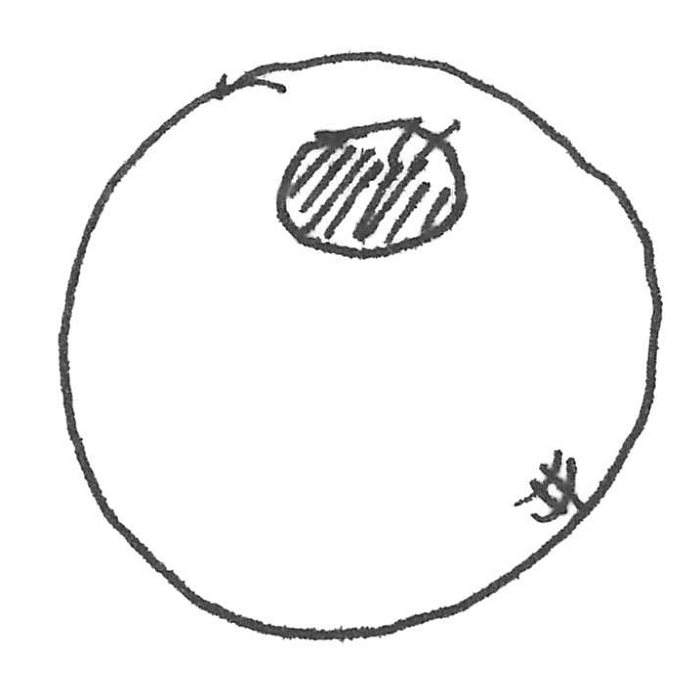
\includegraphics[height=5cm]{fig/normals-patch}
		\caption{\label{fig:normals-patch}Possible normals on $\mathbb{S}^2$}
	\end{subfigure}
	\begin{subfigure}{0.45\columnwidth}
		\centering
		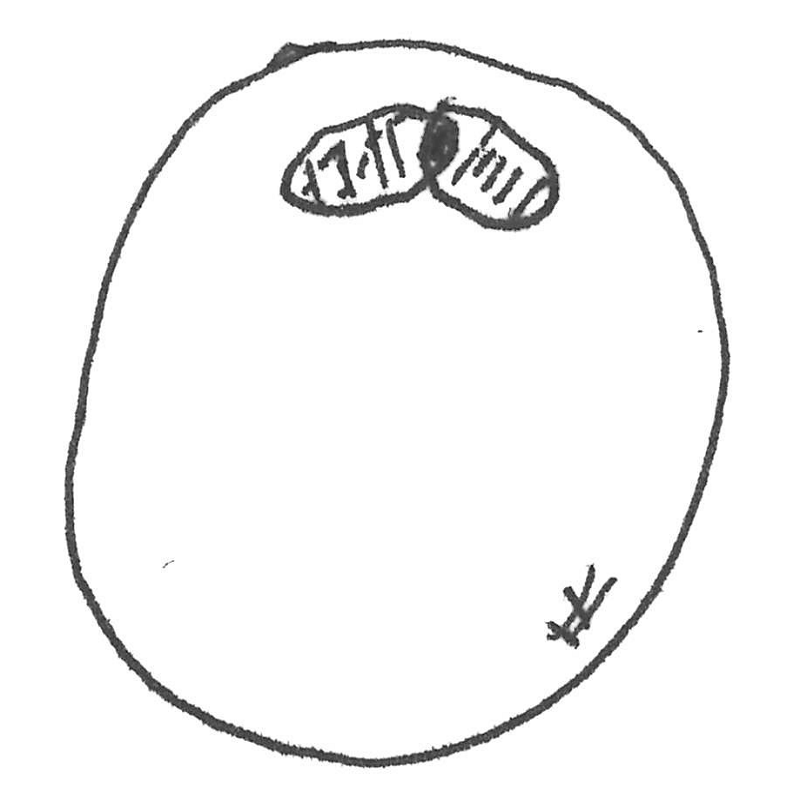
\includegraphics[height=5cm]{fig/normals-patch-intersect}
		\caption{\label{fig:normals-patch-intersection}Overlapping possible normals on $\mathbb{S}^2$}
	\end{subfigure}
	\caption{\label{fig:normals-distrib} Patches on $\mathbb{S}^2$ representing possible
		normals for a critical point. In (b) it's possible for the two points to be paired
		as their normals could be the same, but additional computation is required to
		determine if this is actually the case.}
\end{figure}

In the case of the elevation function on proteins, it is possible the function is not Morse,
making the analysis more challenging. However, these degeneracies capture important
information about the protein structure which would be lost if perturbed, and must be handled
separately. The four possible degenerate cases are shown in \cref{fig:protein-legs}.

\begin{figure}
	\centering
	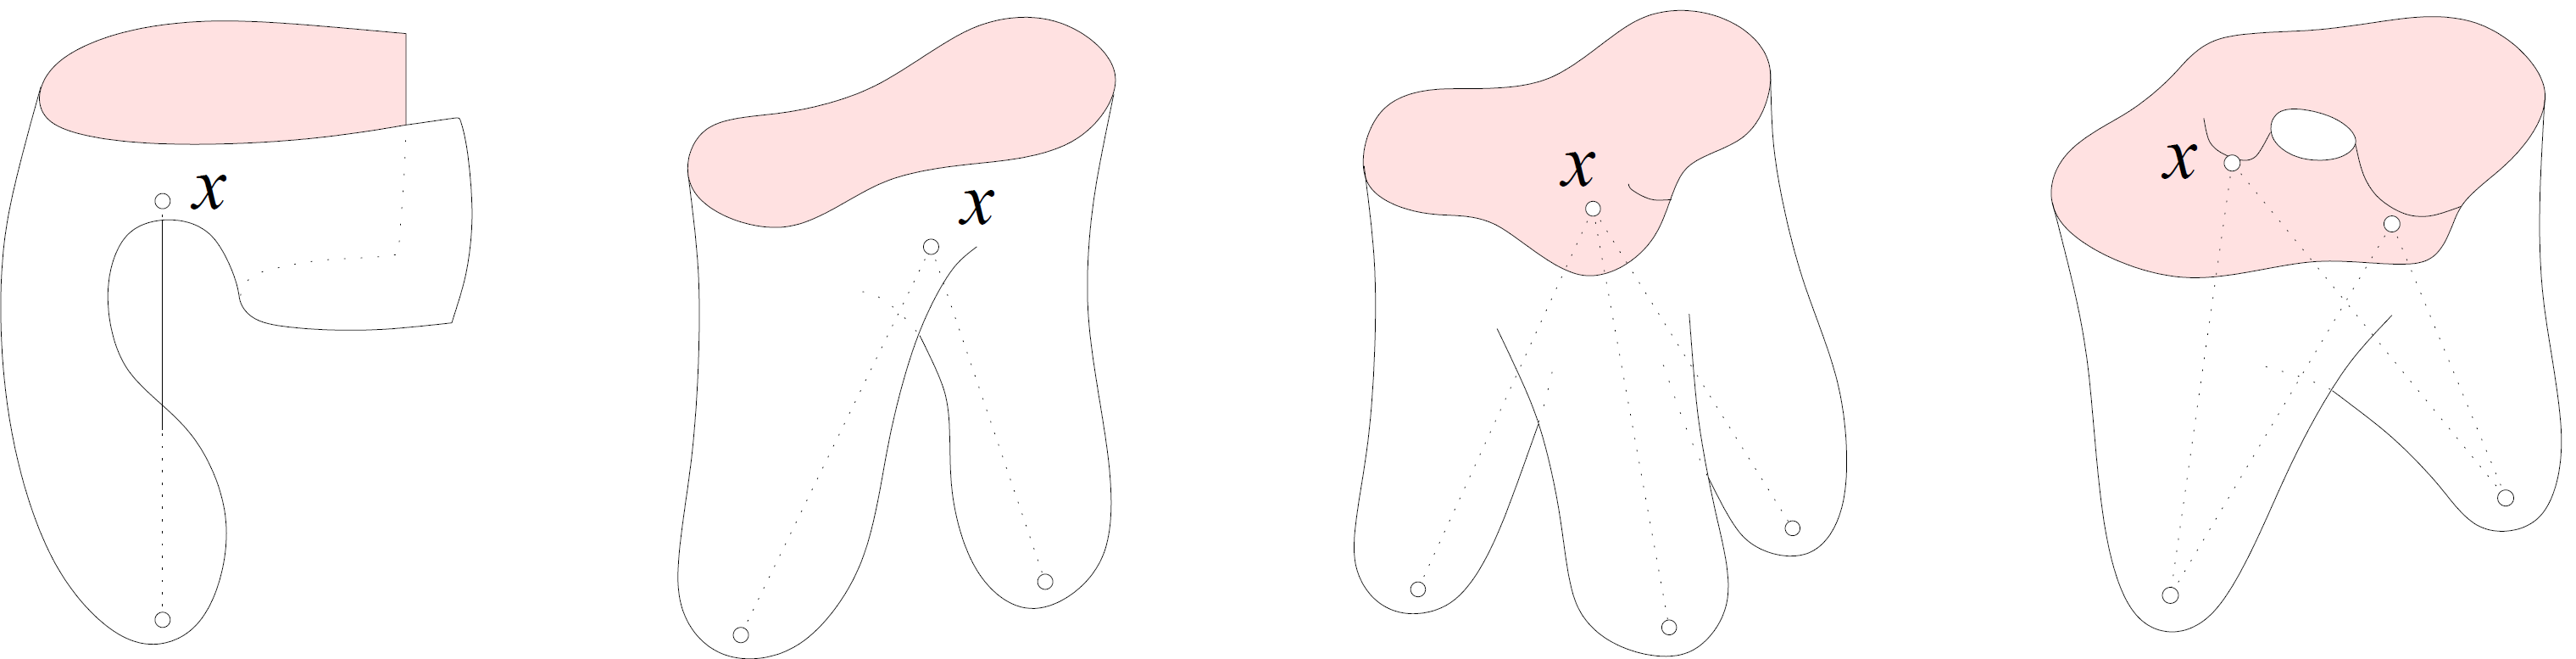
\includegraphics[width=\textwidth]{fig/protein-leg-cases}
	\caption{\label{fig:protein-legs} The possible special cases for protein docking, where
	critical points have equal elevation. From left to right are the one-, two-,
	three- and four-legged cases~\cite{WABER05}. In the two-legged case the saddle $x$
	projects on to the line between the two minima. In the three-legged case it projects
	to the triangle formed by the three minima. In the four-legged case the line between
	the two saddle points can be projected down and will intersect the line between the
	two minima}
\end{figure}

\section*{References}
\beginrefs

% Unsure why she doesn't just want to use bibtex but ok
\bibentry{WABER05}\textsc{Y.~Wang}, \textsc{P.K.~Agarwal}, \textsc{P.~Brown},
\textsc{H.~Edelsbrunner} and \textsc{J.~Rudolph}
``Coarse and Reliable Geometric Alignment for Protein Docking''
\textit{Pacific Symposium on Biocomputing},
2005

\endrefs

\end{document}

